\subsection{Reference Monitor}

\begin{quote}\emph{aka Policy Enforcement Point}\end{quote}

Das \emph{Reference Monitor} Pattern beschreibt eine abstrakte Vorghensweise, wie definierte Sicherheitsvorschriften um- und vorallem durchgesetzt werden können.

\subsection*{Kontext}
Ein IT-System, in welchem Subjekte (Benutzer als auch technische Prozesse) auf diverse Resourcen zugriefen möchten.

\subsection*{Problem}
Die vorangegangenen Patterns beschrieben bis anhin lediglich, \emph{wie} Sicherheitsrichtlinien modelliert und definiert werden können.
Regeln nur zu definieren kommt einem weglassen dieser gleich. Wir benötigen also eine Möglichkeit, die aufgestellten Regeln auch effektiv durchzusetzen und zu überwachen.

Beim definieren eines möglichen Mechanismus soll darauf geachtet werden, dass dieser so abstrakt wie möglich und dadurch auf verschiedenste Architekturen sowie auf alle Ebenen eines Systems appliziert werden kann.

\subsection*{Lösung}
Folgendes Klassendiagramm zeigt den Ansatz des abstrakten \emph{Reference Monitors}, inkl. einer konkreten Implementierung dessen.
Die Collection aus \emph{Authorization Rules} ist konkret mit einer \gls{ACL} vergleichbar.

\begin{figure}[H]
	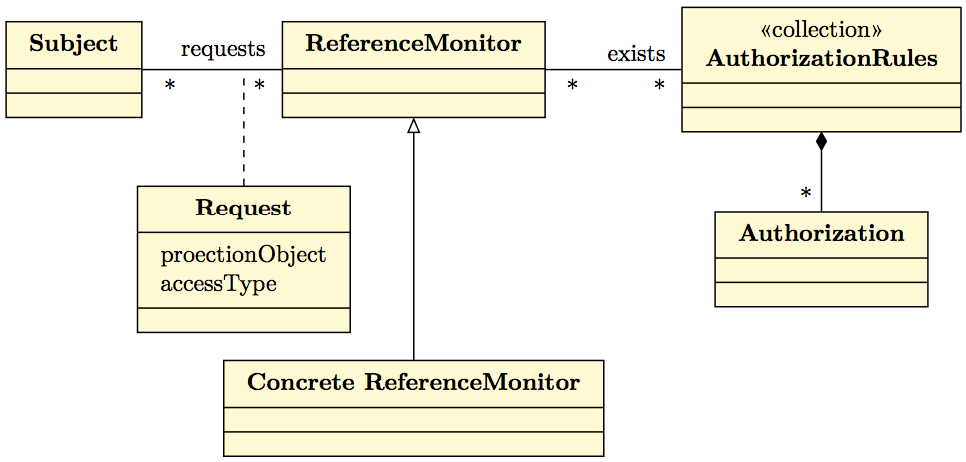
\includegraphics[width=\textwidth]{content/security/accesscontrolmodels/images/referencemonitor.png}
\caption{Reference Monitor - Klassendiagramm}
\end{figure}

Die effektive Überprüfung, ob ein Subjekt für den Zugriff berechtigt ist, ist denkbar einfach: Jeder Zugriff auf eine Resource (ein Protection Object) wird durch den Reference Monitor geführt. Dieser prüft, ob eine entsprechende Zugriffsregel vorhanden ist und gewährt ggf. den Zugriff.

\begin{figure}[H]
	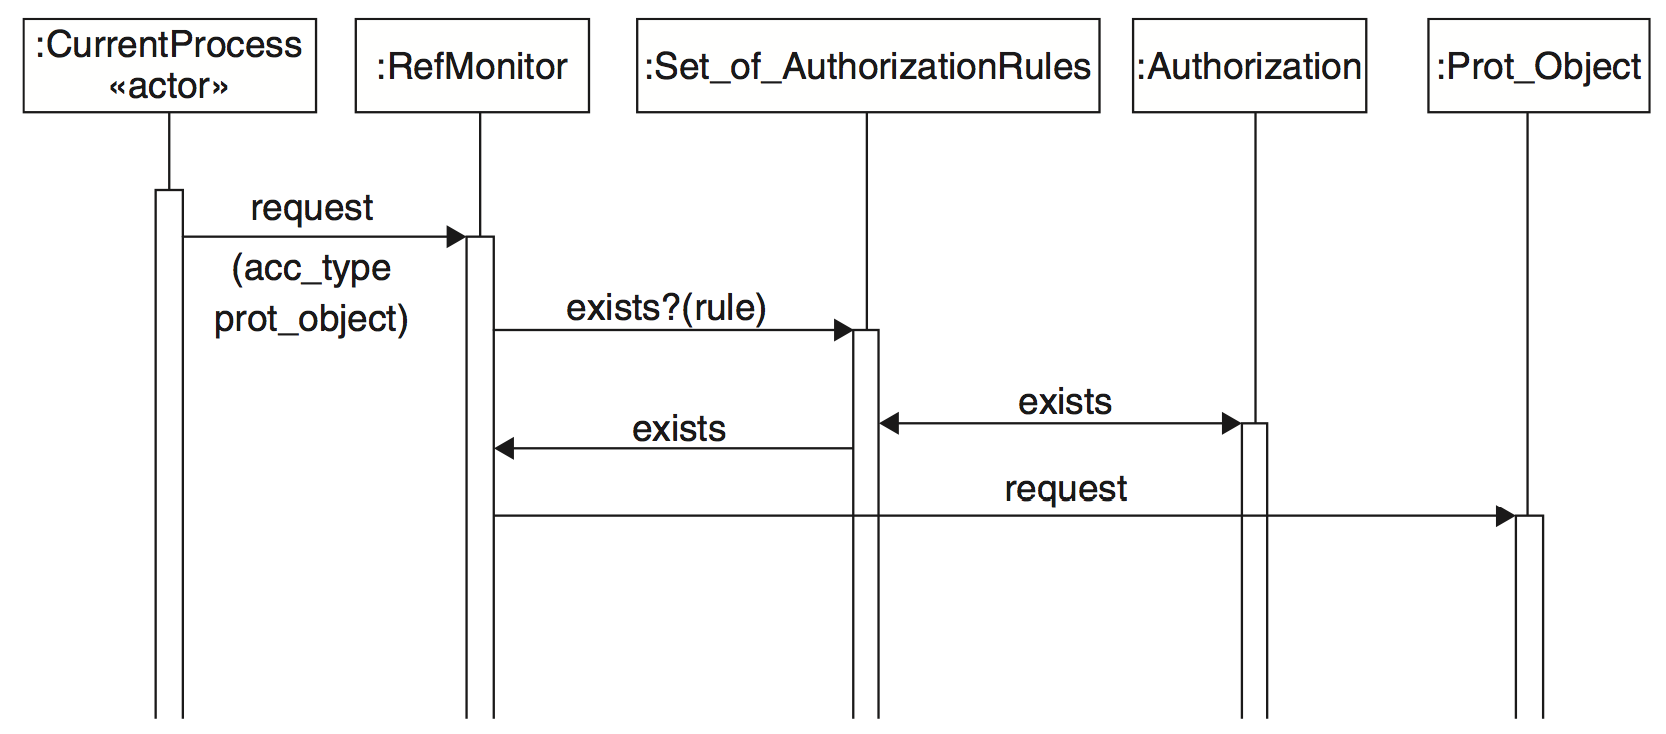
\includegraphics[width=\textwidth]{content/security/accesscontrolmodels/images/referencemonitor_sequence.png}
	\caption{Reference Monitor - Sequenzdiagramm \cite{SecPatterns06}}
\end{figure}

Dieses Vorgehen leitet vom \emph{Interceptor} Pattern ab, und findet an vielen anderen Orten Verwendung (JEE Servlet Filter usw.)


\subsection*{Vor- \& Nachteile}
\begin{itemize}
	\item Wenn sichergestellt werden kann, dass alle \emph{Requests} überprüft werden können, so ist eine maximale Befriedigung der Sicherheitsanforderungen gewährt.
	\item Jede Resource benötigt ihre eigene Implementierung eines \emph{Reference Monitors}; Ein \emph{Request} auf eine Datei muss evtl. anders behandelt werden als ein \emph{Request} auf eine spezifische Datenbanktabelle.
	\item Die Prüfung vieler \emph{Requests} kann bei hoher Systemlast zum Performancerisiko führen. Dementsprechend sollte die Logik zur Sicherheitsprüfung auch so einfach/schlank wie möglich gehalten werden.
\end{itemize}

\subsection*{Beispielanwendungen}
\begin{itemize}
	\item Datenbanksysteme
	\item Betriebsysteme (bspw. Windows 2000 ff. verwendet eine ACL für NTFS Berechtigungen)
\end{itemize}